\documentclass{standalone}
\usepackage{tikz}
\usetikzlibrary{patterns, positioning}


\begin{document}
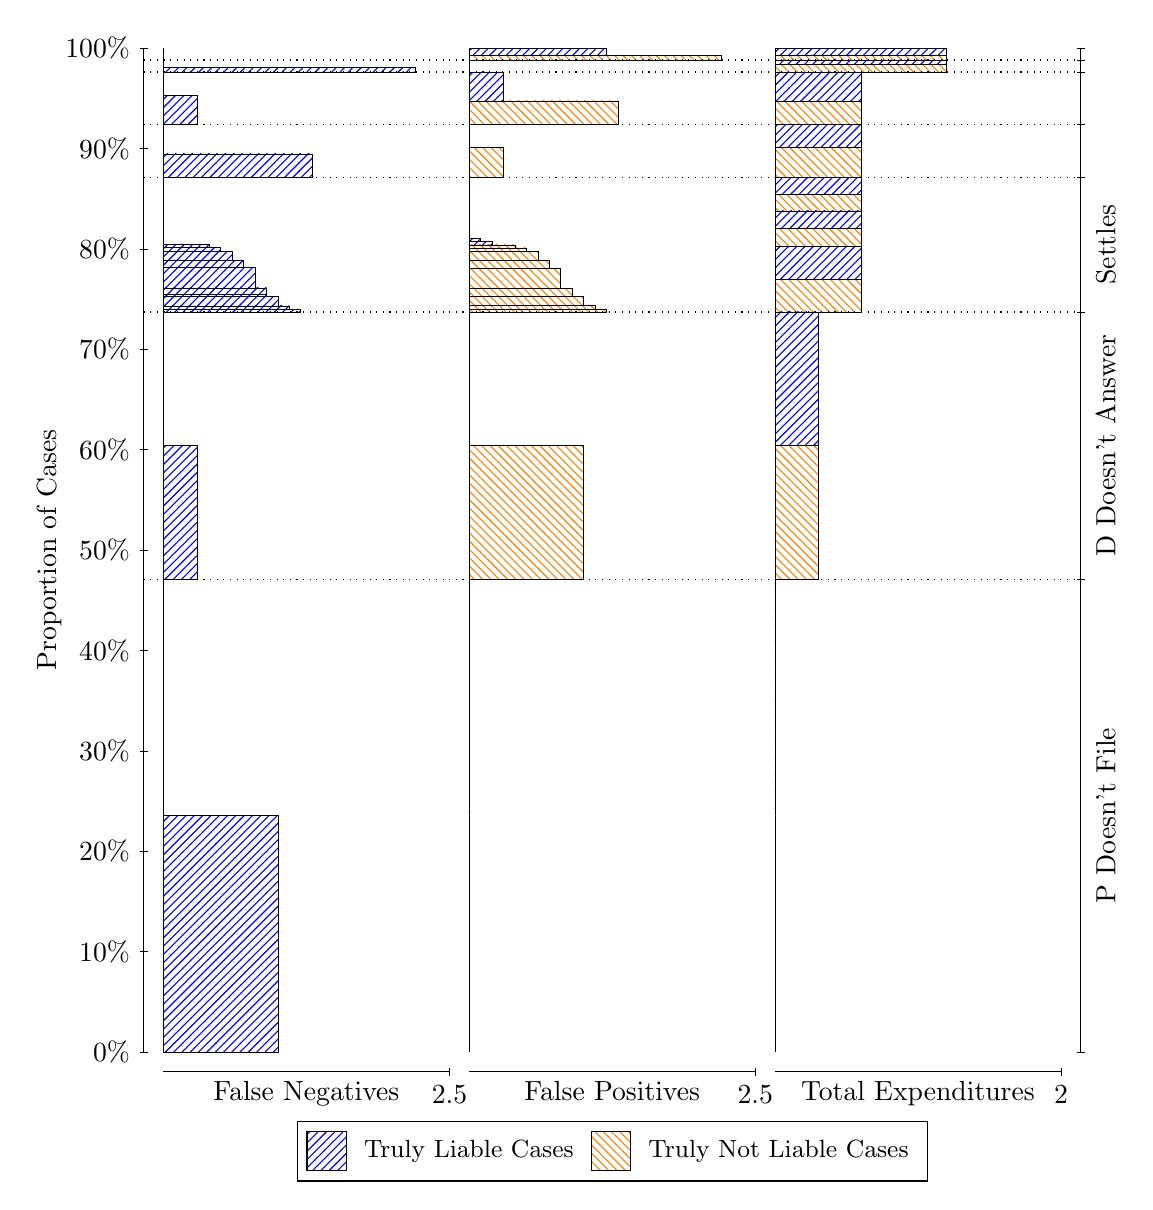
\begin{tikzpicture}
\draw[black, very thin] (1.5,1.75) -- (1.5,14.5);
\node[rotate=90, text=black, anchor=center] at (0.3, 8.125) {Proportion of Cases};
\draw[black, very thin] (1.45,1.75) -- (1.55,1.75);
\node[text=black, anchor=east] at (1.45, 1.75) {0\%};
\draw[black, very thin] (1.45,3.025) -- (1.55,3.025);
\node[text=black, anchor=east] at (1.45, 3.025) {10\%};
\draw[black, very thin] (1.45,4.3) -- (1.55,4.3);
\node[text=black, anchor=east] at (1.45, 4.3) {20\%};
\draw[black, very thin] (1.45,5.575) -- (1.55,5.575);
\node[text=black, anchor=east] at (1.45, 5.575) {30\%};
\draw[black, very thin] (1.45,6.85) -- (1.55,6.85);
\node[text=black, anchor=east] at (1.45, 6.85) {40\%};
\draw[black, very thin] (1.45,8.125) -- (1.55,8.125);
\node[text=black, anchor=east] at (1.45, 8.125) {50\%};
\draw[black, very thin] (1.45,9.4) -- (1.55,9.4);
\node[text=black, anchor=east] at (1.45, 9.4) {60\%};
\draw[black, very thin] (1.45,10.675) -- (1.55,10.675);
\node[text=black, anchor=east] at (1.45, 10.675) {70\%};
\draw[black, very thin] (1.45,11.95) -- (1.55,11.95);
\node[text=black, anchor=east] at (1.45, 11.95) {80\%};
\draw[black, very thin] (1.45,13.225) -- (1.55,13.225);
\node[text=black, anchor=east] at (1.45, 13.225) {90\%};
\draw[black, very thin] (1.45,14.5) -- (1.55,14.5);
\node[text=black, anchor=east] at (1.45, 14.5) {100\%};

\draw[black, very thin] (13.4,1.75) -- (13.4,14.5);
\draw[black, very thin] (13.35,1.75) -- (13.45,1.75);
\node[anchor=west] at (13.35, 1.75) {};
\draw[black, very thin] (13.35,7.7515) -- (13.45,7.7515);
\node[anchor=west] at (13.35, 7.7515) {};
\draw[black, very thin] (13.35,11.148) -- (13.45,11.148);
\node[anchor=west] at (13.35, 11.148) {};
\draw[black, very thin] (13.35,12.861) -- (13.45,12.861);
\node[anchor=west] at (13.35, 12.861) {};
\draw[black, very thin] (13.35,13.534) -- (13.45,13.534);
\node[anchor=west] at (13.35, 13.534) {};
\draw[black, very thin] (13.35,14.195) -- (13.45,14.195);
\node[anchor=west] at (13.35, 14.195) {};
\draw[black, very thin] (13.35,14.348) -- (13.45,14.348);
\node[anchor=west] at (13.35, 14.348) {};
\draw[black, very thin] (13.35,14.5) -- (13.45,14.5);
\node[anchor=west] at (13.35, 14.5) {};

\draw[black, very thin, pattern color=blue, pattern=north east lines] (1.75,1.75) rectangle (3.2033,4.7508);
\draw[black, very thin, pattern color=orange, pattern=north west lines] (1.75,4.7508) rectangle (1.75,7.7515);
\draw[black, very thin, pattern color=blue, pattern=north east lines] (1.75,7.7515) rectangle (2.186,9.4496);
\draw[black, very thin, pattern color=orange, pattern=north west lines] (1.75,9.4496) rectangle (1.75,11.148);
\draw[black, very thin, pattern color=blue, pattern=north east lines] (1.75,11.148) rectangle (3.494,11.185);
\draw[black, very thin, pattern color=blue, pattern=north east lines] (1.75,11.185) rectangle (3.3487,11.226);
\draw[black, very thin, pattern color=blue, pattern=north east lines] (1.75,11.226) rectangle (3.2033,11.346);
\draw[black, very thin, pattern color=blue, pattern=north east lines] (1.75,11.346) rectangle (3.058,11.371);
\draw[black, very thin, pattern color=blue, pattern=north east lines] (1.75,11.371) rectangle (3.058,11.453);
\draw[black, very thin, pattern color=blue, pattern=north east lines] (1.75,11.453) rectangle (2.9127,11.711);
\draw[black, very thin, pattern color=blue, pattern=north east lines] (1.75,11.711) rectangle (2.7673,11.807);
\draw[black, very thin, pattern color=blue, pattern=north east lines] (1.75,11.807) rectangle (2.622,11.922);
\draw[black, very thin, pattern color=blue, pattern=north east lines] (1.75,11.922) rectangle (2.4767,11.968);
\draw[black, very thin, pattern color=blue, pattern=north east lines] (1.75,11.968) rectangle (2.3313,12.008);
\draw[black, very thin, pattern color=orange, pattern=north west lines] (1.75,12.008) rectangle (1.75,12.861);
\draw[black, very thin, pattern color=blue, pattern=north east lines] (1.75,12.861) rectangle (3.6393,13.157);
\draw[black, very thin, pattern color=orange, pattern=north west lines] (1.75,13.157) rectangle (1.75,13.534);
\draw[black, very thin, pattern color=blue, pattern=north east lines] (1.75,13.534) rectangle (2.186,13.901);
\draw[black, very thin, pattern color=orange, pattern=north west lines] (1.75,13.901) rectangle (1.75,14.195);
\draw[black, very thin, pattern color=blue, pattern=north east lines] (1.75,14.195) rectangle (4.9473,14.25);
\draw[black, very thin, pattern color=orange, pattern=north west lines] (1.75,14.25) rectangle (1.75,14.348);
\draw[black, very thin, pattern color=orange, pattern=north west lines] (1.75,14.348) rectangle (1.75,14.402);
\draw[black, very thin, pattern color=blue, pattern=north east lines] (1.75,14.402) rectangle (1.75,14.5);
\draw[black, very thin, pattern color=orange, pattern=north west lines] (5.6333,1.75) rectangle (5.6333,4.7508);
\draw[black, very thin, pattern color=blue, pattern=north east lines] (5.6333,4.7508) rectangle (5.6333,7.7515);
\draw[black, very thin, pattern color=orange, pattern=north west lines] (5.6333,7.7515) rectangle (7.0867,9.4496);
\draw[black, very thin, pattern color=blue, pattern=north east lines] (5.6333,9.4496) rectangle (5.6333,11.148);
\draw[black, very thin, pattern color=orange, pattern=north west lines] (5.6333,11.148) rectangle (7.3773,11.185);
\draw[black, very thin, pattern color=orange, pattern=north west lines] (5.6333,11.185) rectangle (7.232,11.227);
\draw[black, very thin, pattern color=orange, pattern=north west lines] (5.6333,11.227) rectangle (7.0867,11.347);
\draw[black, very thin, pattern color=orange, pattern=north west lines] (5.6333,11.347) rectangle (6.9413,11.451);
\draw[black, very thin, pattern color=orange, pattern=north west lines] (5.6333,11.451) rectangle (6.796,11.704);
\draw[black, very thin, pattern color=orange, pattern=north west lines] (5.6333,11.704) rectangle (6.6507,11.799);
\draw[black, very thin, pattern color=orange, pattern=north west lines] (5.6333,11.799) rectangle (6.5053,11.915);
\draw[black, very thin, pattern color=orange, pattern=north west lines] (5.6333,11.915) rectangle (6.36,11.962);
\draw[black, very thin, pattern color=orange, pattern=north west lines] (5.6333,11.962) rectangle (6.2147,12);
\draw[black, very thin, pattern color=blue, pattern=north east lines] (5.6333,12) rectangle (5.924,12.041);
\draw[black, very thin, pattern color=blue, pattern=north east lines] (5.6333,12.041) rectangle (5.7787,12.086);
\draw[black, very thin, pattern color=blue, pattern=north east lines] (5.6333,12.086) rectangle (5.6333,12.861);
\draw[black, very thin, pattern color=orange, pattern=north west lines] (5.6333,12.861) rectangle (6.0693,13.238);
\draw[black, very thin, pattern color=blue, pattern=north east lines] (5.6333,13.238) rectangle (5.6333,13.534);
\draw[black, very thin, pattern color=orange, pattern=north west lines] (5.6333,13.534) rectangle (7.5227,13.828);
\draw[black, very thin, pattern color=blue, pattern=north east lines] (5.6333,13.828) rectangle (6.0693,14.195);
\draw[black, very thin, pattern color=orange, pattern=north west lines] (5.6333,14.195) rectangle (5.6333,14.293);
\draw[black, very thin, pattern color=blue, pattern=north east lines] (5.6333,14.293) rectangle (5.6333,14.348);
\draw[black, very thin, pattern color=orange, pattern=north west lines] (5.6333,14.348) rectangle (8.8307,14.402);
\draw[black, very thin, pattern color=blue, pattern=north east lines] (5.6333,14.402) rectangle (7.3773,14.5);
\draw[black, very thin, pattern color=orange, pattern=north west lines] (9.5167,1.75) rectangle (9.5167,4.7508);
\draw[black, very thin, pattern color=blue, pattern=north east lines] (9.5167,4.7508) rectangle (9.5167,7.7515);
\draw[black, very thin, pattern color=orange, pattern=north west lines] (9.5167,7.7515) rectangle (10.062,9.4496);
\draw[black, very thin, pattern color=blue, pattern=north east lines] (9.5167,9.4496) rectangle (10.062,11.148);
\draw[black, very thin, pattern color=orange, pattern=north west lines] (9.5167,11.148) rectangle (10.607,11.564);
\draw[black, very thin, pattern color=blue, pattern=north east lines] (9.5167,11.564) rectangle (10.607,11.982);
\draw[black, very thin, pattern color=orange, pattern=north west lines] (9.5167,11.982) rectangle (10.607,12.208);
\draw[black, very thin, pattern color=blue, pattern=north east lines] (9.5167,12.208) rectangle (10.607,12.431);
\draw[black, very thin, pattern color=orange, pattern=north west lines] (9.5167,12.431) rectangle (10.607,12.642);
\draw[black, very thin, pattern color=blue, pattern=north east lines] (9.5167,12.642) rectangle (10.607,12.861);
\draw[black, very thin, pattern color=orange, pattern=north west lines] (9.5167,12.861) rectangle (10.607,13.238);
\draw[black, very thin, pattern color=blue, pattern=north east lines] (9.5167,13.238) rectangle (10.607,13.534);
\draw[black, very thin, pattern color=orange, pattern=north west lines] (9.5167,13.534) rectangle (10.607,13.828);
\draw[black, very thin, pattern color=blue, pattern=north east lines] (9.5167,13.828) rectangle (10.607,14.195);
\draw[black, very thin, pattern color=orange, pattern=north west lines] (9.5167,14.195) rectangle (11.697,14.293);
\draw[black, very thin, pattern color=blue, pattern=north east lines] (9.5167,14.293) rectangle (11.697,14.348);
\draw[black, very thin, pattern color=orange, pattern=north west lines] (9.5167,14.348) rectangle (11.697,14.402);
\draw[black, very thin, pattern color=blue, pattern=north east lines] (9.5167,14.402) rectangle (11.697,14.5);
\draw[black, dotted] (1.5,7.7515) -- (13.4,7.7515);
\draw[black, dotted] (1.5,11.148) -- (13.4,11.148);
\draw[black, dotted] (1.5,12.861) -- (13.4,12.861);
\draw[black, dotted] (1.5,13.534) -- (13.4,13.534);
\draw[black, dotted] (1.5,14.195) -- (13.4,14.195);
\draw[black, dotted] (1.5,14.348) -- (13.4,14.348);
\draw[black, very thin] (1.75,1.5) -- (5.3833,1.5);
\node[text=black, anchor=north] at (3.5667, 1.5) {False Negatives};
\draw[black, very thin] (5.3833,1.45) -- (5.3833,1.55);
\node[text=black, anchor=north] at (5.3833, 1.45) {2.5};

\draw[black, very thin] (5.6333,1.5) -- (9.2667,1.5);
\node[text=black, anchor=north] at (7.45, 1.5) {False Positives};
\draw[black, very thin] (9.2667,1.45) -- (9.2667,1.55);
\node[text=black, anchor=north] at (9.2667, 1.45) {2.5};

\draw[black, very thin] (9.5167,1.5) -- (13.15,1.5);
\node[text=black, anchor=north] at (11.333, 1.5) {Total Expenditures};
\draw[black, very thin] (13.15,1.45) -- (13.15,1.55);
\node[text=black, anchor=north] at (13.15, 1.45) {2};

\node[text=black, centered, rotate=90] at (13.72, 4.7508) {P Doesn't File};
\node[text=black, centered, rotate=90] at (13.72, 9.4496) {D Doesn't Answer};
\node[text=black, centered, rotate=90] at (13.72, 12.004) {Settles};





\draw (7.449999999999999,1.5) node[draw=none] (baseCoordinate) {};
\begin{scope}[align=center]
        \matrix[scale=0.5, draw=black, below=0.5cm of baseCoordinate, nodes={draw}, column sep=0.1cm]{
            \node[rectangle, draw, minimum width=0.5cm, minimum height=0.5cm, pattern color=blue, pattern=north east lines] {}; &
            \node[draw=none, font=\small, text=black] (B) {Truly Liable Cases}; &
            \node[rectangle, draw, minimum width=0.5cm, minimum height=0.5cm, pattern color=orange, pattern=north west lines] {}; &
            \node[draw=none, font=\small, text=black] (B) {Truly Not Liable Cases}; \\
            };
\end{scope}

\end{tikzpicture}
\end{document}